\documentclass{article}

\usepackage[utf8]{inputenc}   %for german letters ä,ö...
\usepackage[english]{babel}   %german settings
\usepackage{amsmath}
\usepackage{amssymb}
\usepackage{tikz,pgfplots}
\usetikzlibrary{patterns}
\usepackage[justification=centering]{caption}
\usepackage[left=2.5cm,right=2.5cm,top=2cm,bottom=3cm]{geometry}
\usepackage[tight-spacing=true]{siunitx}
\usepackage{booktabs}
\usepackage[outdir=./]{epstopdf}
\usepackage{subcaption}
\usepackage{placeins}
\usepackage{esdiff}

\usepackage{mathrsfs}
\usetikzlibrary{arrows,decorations.pathmorphing}
\newcommand{\degre}{\ensuremath{^\circ}}

\usetikzlibrary{patterns}
\tikzstyle{spring}=[thick,decorate,decoration={zigzag,pre length=0.3cm,post length=0.3cm,segment length=6}]

\sisetup{locale = UK}

\newcommand{\upd}[1]{^\mathrm{#1}}
\newcommand{\ind}[1]{_\mathrm{#1}}
\newcommand{\RM}[1]{\MakeUppercase{\romannumeral #1}}


\usepackage[backend=bibtex8,sorting=none]{biblatex}
\addbibresource{refs.bib}

\begin{document}
\setlength{\parindent}{0em}   %Einrücken verhindern
\title{Advanced Laboratory Course\\Experiment K225\\Positron Lifetime in Metals and Insulators}
\author{Kilian Bönisch \ \ \ \qquad s6kiboen@uni-bonn.de \qquad 2897138\\
  Friedrich Hübner \qquad s6frhueb@uni-bonn.de \qquad 2897111}
\date{05.09.18}

\maketitle
\thispagestyle{empty}

\newpage

\thispagestyle{empty}

\tableofcontents

\newpage

\section{Introduction}

In this experiment we measure the transport properties of copper. This includes the electrical resistivity, the thermal conductivity and the temperature dependence of the Hall Effect of copper.

\section{Theoretical Background}

\subsection{Magnetoresistance}
The electrical properties of metals change when an external magnetic field $\vec{B}$ is applied. It should be noted that we only consider the transverse magneto resistance, although there will also be a longitudinal magnetoresistance. In a simple model for the transverse magnetoresistance, the metal consists of two charge carriers, e.\ g.\ electrons and holes. Both types contribute to the total current
\begin{align*}
    \vec{j}_\mathrm{tot}=\vec{j}_1+\vec{j}_2.
\end{align*}
Both charge carriers have a corresponding resistivity inversely proportional to the conductivity
\begin{align*}
    \rho_i=\frac{1}{\sigma_i}.
\end{align*}
The total resistivity is then given by 
\begin{align*}
    \rho=\frac{1}{\sigma_1+\sigma_2}.
\end{align*}
For the dependence of the external magnetic field we are interested in the change of the resistivity
\begin{align*}
    \Delta \rho=\rho-\rho_0,
\end{align*}
where $\rho_0$ is the zero field ($B=0$) resistivity. According to Kohlers Rule one then has the functional relationship
\begin{align}
    \frac{\Delta \rho}{\rho_0}=F\left( \frac{B}{\rho_0} \right)
    \label{eq:kohler_1}
\end{align}
for some function $F$ which only depends on the metal.\\ 

To measure the resistivity of copper the 4-point method is used in order to not measure the dominating rersistance of the wires and contacts. The resistivity can then be calculated by
\begin{align*}
    \rho=\frac{AU_\mathrm{R}}{I_\mathrm{R}l_\mathrm{R}},
\end{align*}
where $A$ is the cross-sectional area of the sample, $U_\mathrm{R}$ is the voltage measured over the distance $l_\mathrm{R}$ and $I_\mathrm{R}$ is the applied current.

\subsection{Thermal Conductivity}
The thermal conductivity of a metal also changes when an external magnetic field is applied. This can be understood by considering the deflection of the electrons due to the Lorentz force. Equivalent to \ref{eq:kohler_1} Kohler proposed that for the thermal conductivity
\begin{align*}
    \frac{\Delta \kappa}{\kappa}=G \left( \frac{B\kappa_0}{T} \right)
\end{align*}
holds for some function $G$ depending on the metal only.

\section{Procedure}

The setup of the two lasers, including the setup for the polarization spectroscopy, is already adjusted and can be seen in figure \ref{fig:setup_laser}.

\begin{figure}[h]
  \centering
  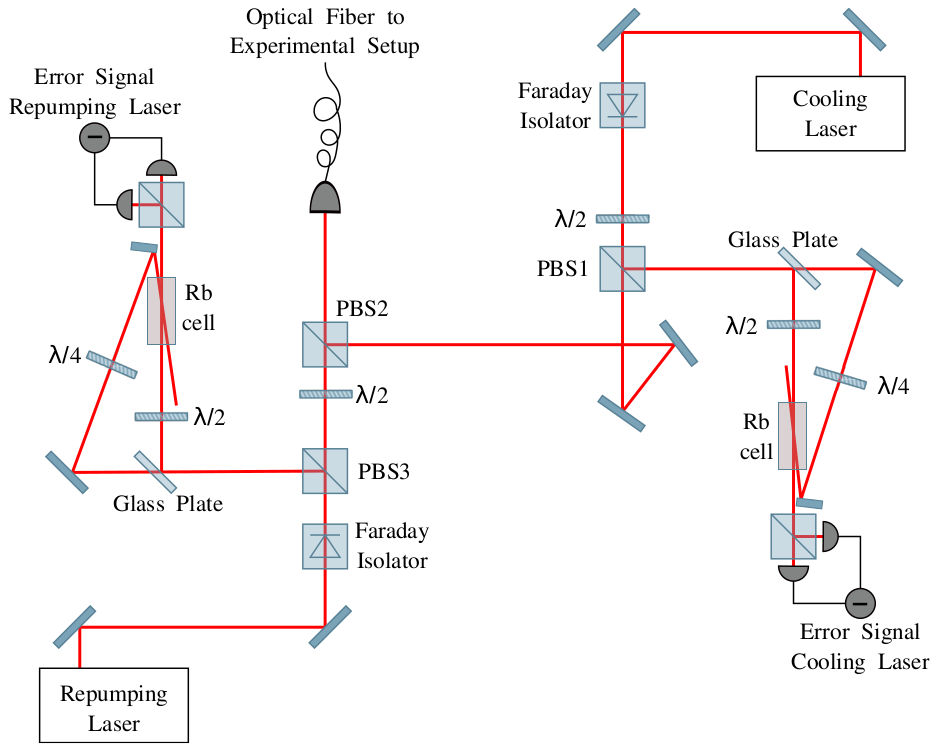
\includegraphics[width=0.5\textwidth]{figures/setup_laser.png}
  \caption{Setup of the pump laser and the cooling laser.}
  \label{fig:setup_laser}
\end{figure}

With an optical fibre the two beams get to the actual setup of the MOT which can be seen in figure \ref{fig:setup_mot}.

\begin{figure}[h]
  \centering
  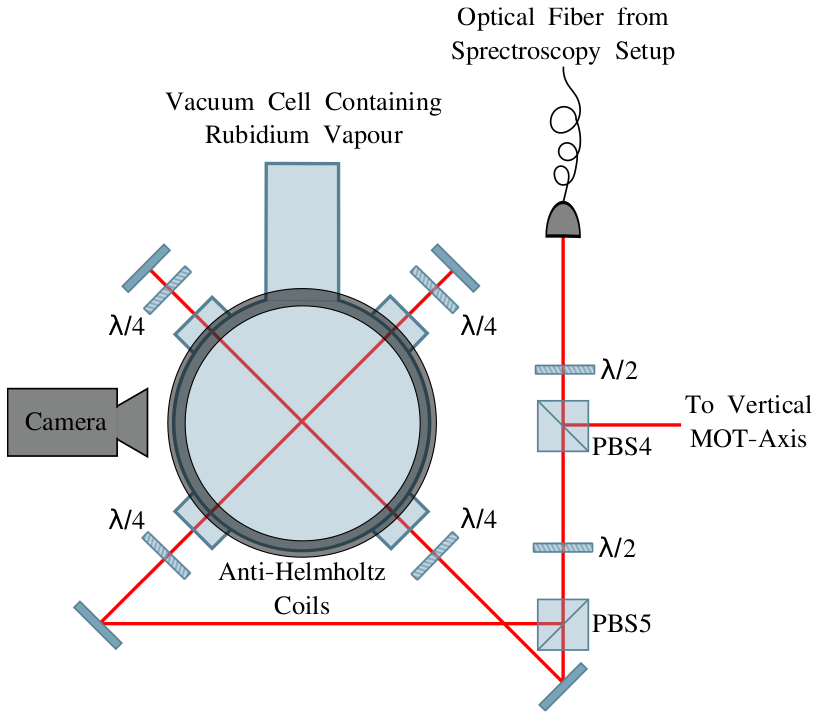
\includegraphics[width=0.5\textwidth]{figures/setup_mot.png}
  \caption{Alignment of the lasers in the MOT.}
  \label{fig:setup_mot}
\end{figure}

\subsection{Adjustment of the Beams}
As a first step we adjust the alignment of the beams in figure \ref{fig:setup_mot}. It is important that the beams cross each other in the center of the quadrupole field. This can be checked with the camera es the tutor showed us where the beams should cross each other on the display. With a CCD-camera\footnote{With the camera we can see the fluorescence of the rubidium atoms in the chamber.} we make sure that the beams really cross in one point. Using an aperture we make sure that each reflected beam is parallel to the original beam. A picture of the resulting setup can be seen in figure ???.\\ \\

???\\ \\

Additionally one must make sure that the power of the laser is split into three equal parts (for each axis). To do so we measure the power of each of the three beams with the powermeter. Adjusting the $\lambda/2$-plates we get an equal intensity of about \SI{1.2}{\milli\watt} per axis (in the original laser setup). This adjustment is done with the pumping laser turned of as we are only interested in the intensity of the cooling laser beeing equal for each axis. 


\section{Evaluation}

\section{Part 1}
\subsection{Assignment 3 - myon energy loss}

\begin{table}
\centering
\caption{Myon momentum in inner and outer detector}
\begin{tabular}{ccc}
\toprule
n & $p_{in}/\si{GeV}$ & $p_{out}/\si{GeV}$\\
\midrule
1 & / & /\\
2&	-85&	-53.92\\
3&	43.4&	43.83\\
4&	-241.37&	-237.02\\
5&	48.89&	44.77\\
6&	-168.16&	-177.62\\
7&	117.32&	96.56\\
8&	-71.94&	-64.96\\
9&	199.91&	199.44\\
10&	-57.84&	-50.01\\
11&	/ & /\\
12&-100.75&	-94.11\\
13&	38.26&	34.48\\
14&	-105.19&	-108.68\\
15&	236.12&	236.61\\
16&	-131.69&	-125.51\\
17&	152.24&	157.69\\
18&	-35.23&	-32.18\\
19&	54.19&	50\\
20&	-84.75&	-68.09\\
21&	104.26&	107.98\\
22&	-184.01&	-170.66\\
23&	100.36&	101.13\\
\bottomrule
\end{tabular}
\label{tab:task1_myon}
\end{table}

In tabular \ref{tab:task1_myon} the measured momentum in the inner and outer detector part are given for the first 23 events. In event 1 and 11 the myon trace did not continue to the outer part. The energy loss is now given by $\Delta E = |p_out| - |p_in|$ (note that the myons can be treated like relativistic particles). The mean energy loss is given by $\Delta E = \si{5 \pm 9\,GeV}$.

\subsection{Assignment 6 - $Z_0 \to e^+ e^-$ invariant mass}
\begin{table}
\centering
\caption{Electron/positron momentum and the invariant mass $m$}
\begin{tabular}{ccccc}
\toprule
n & $p_1$/GeV & $p_2$/GeV & $m_1$/GeV & $m_2$/GeV\\
\midrule
1 &	-115.81&	63.29 & 171.23 & 171.23\\ 
2&	-49.69&	60.92 & 110.04 & 110.04\\
3&	-78.58&	101.01& 178.18 & 178.18\\
\bottomrule
\end{tabular}
\label{tab:task1_zee}
\end{table}

In tabular \ref{tab:task1_zee} the momentum of the $e^+/e^-$ is given together with the corresponding invariant mass. The invariant mass was calculated in two ways, first using the electron mass and second neglecting the electron mass. As one can see the electron mass does not have an influence on the invariant mass (So the electrons can be treated as ultra relativistic). 

\section{Part 2}
\begin{figure}
\centering
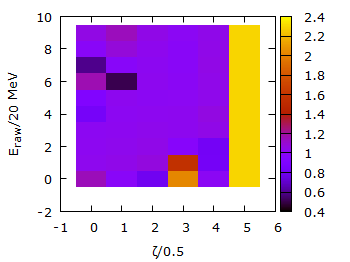
\includegraphics[scale=1]{data/zee_init/zee_init.png}
\caption{Correction factor $E_e/E_{\mathrm{raw}}$ over $E_{\mathrm{raw}}$ and $\eta$}
\label{fig:part2_factor}
\end{figure}

In figure \ref{fig:part2_factor} the correction factor $E_e/E_{\mathrm{raw}}$ is plotted over the raw energy $E_{\mathrm{raw}}$ and $\eta$. 

\section{Part 3 - W Boson mass}

The QCD scale factor was set to $0.33$.

\begin{table}
\centering
\caption{Measured half maxima $h$ for different W boson masses}
\begin{tabular}{ccccc}
\toprule
$m_W$/MeV & $h$/Gev & $\Delta h$/GeV\\ 
\midrule
75&	40.18&	0.06\\
78&	41.78&	0.07\\
79&	42.25&	0.06\\
80&	42.85&	0.06\\
81&	43.46&	0.07\\
82&	43.79&	0.07\\
85&	45.49&	0.11\\
\bottomrule
\end{tabular}
\label{tab:task3_33}
\end{table}

\newpage

\section{Conclusion}

We were able to create a MOT. Unfortunately it was not very stable because the locking of the laser didn't work properly. Using this we were able measure several dependencies of the florescence, e.g. from the quarter waveplates or the magnetic field and we discussed these dependencies. However since our MOT was not stable we needed to redo our MOT every time. Redoing the MOT under equal conditions yields to wide range of values for the florescence.

\FloatBarrier

\newpage

\printbibliography

\newpage

\section{Appendix}

\subsection{Gauge curves}
\begin{figure}
\centering
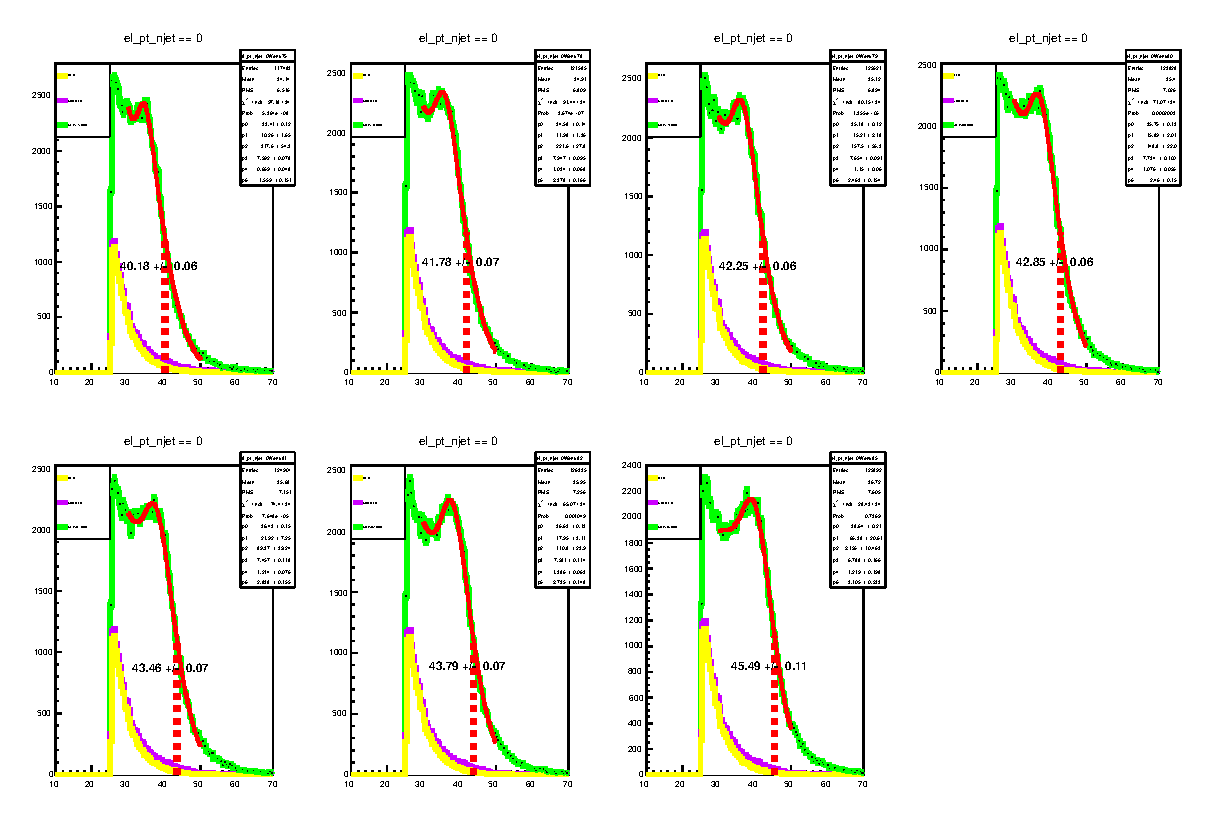
\includegraphics[width=\textwidth]{data/img/gauge_031.eps}
\caption{Gauge measurements for QCD scale factor 0.31 and fit range 30 - 50 GeV}
\end{figure}
\begin{figure}
\centering
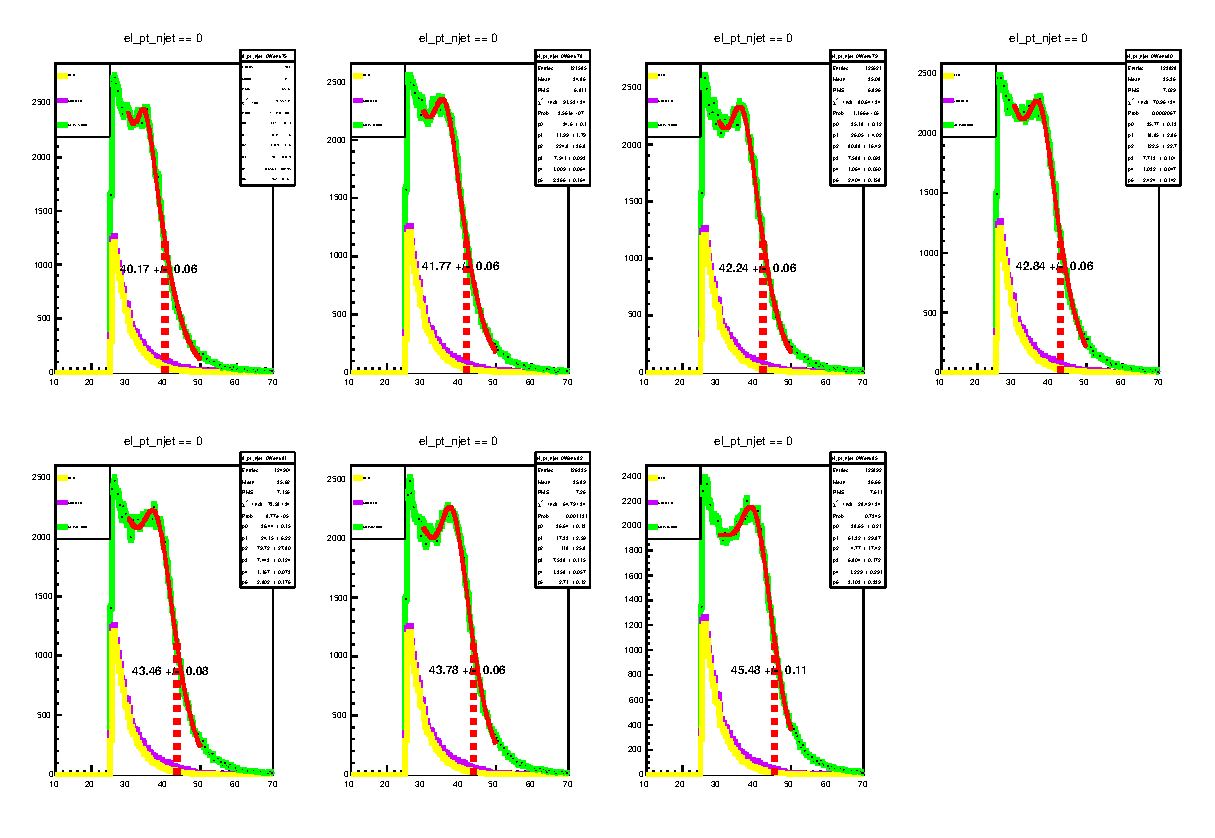
\includegraphics[width=\textwidth]{data/img/gauge_033.eps}
\caption{Gauge measurements for QCD scale factor 0.33 and fit range 30 - 50 GeV}
\end{figure}
\begin{figure}
\centering
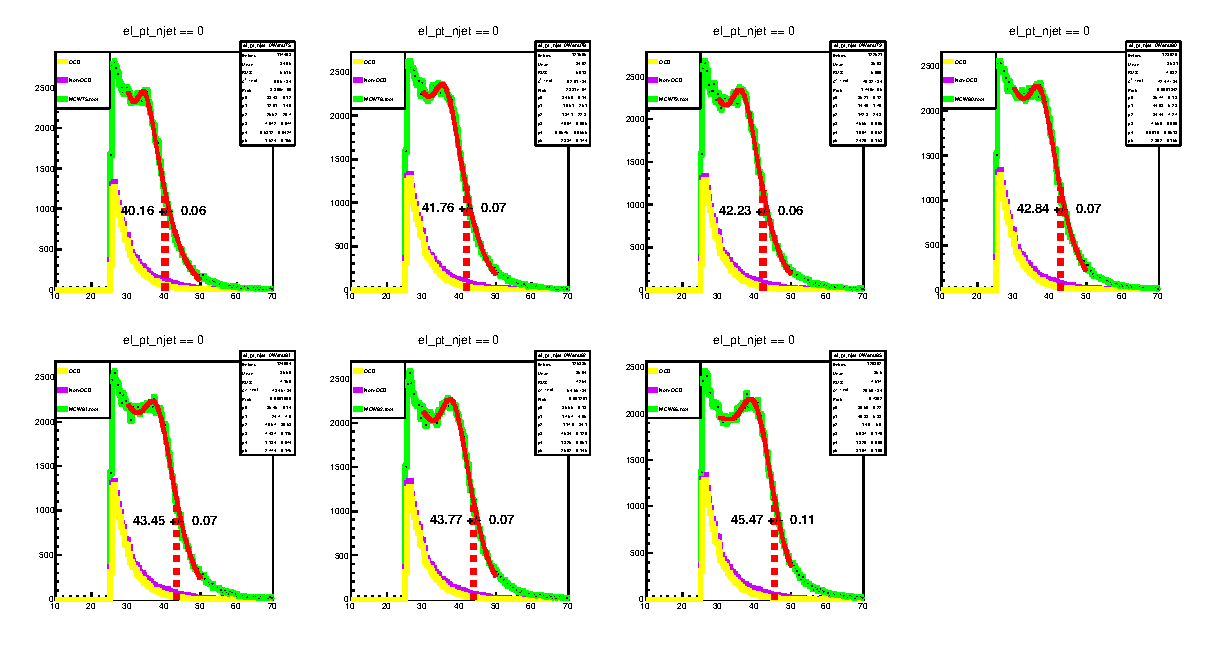
\includegraphics[width=\textwidth]{data/img/gauge_035.eps}
\caption{Gauge measurements for QCD scale factor 0.35 and fit range 30 - 50 GeV}
\end{figure}
\begin{figure}
\centering
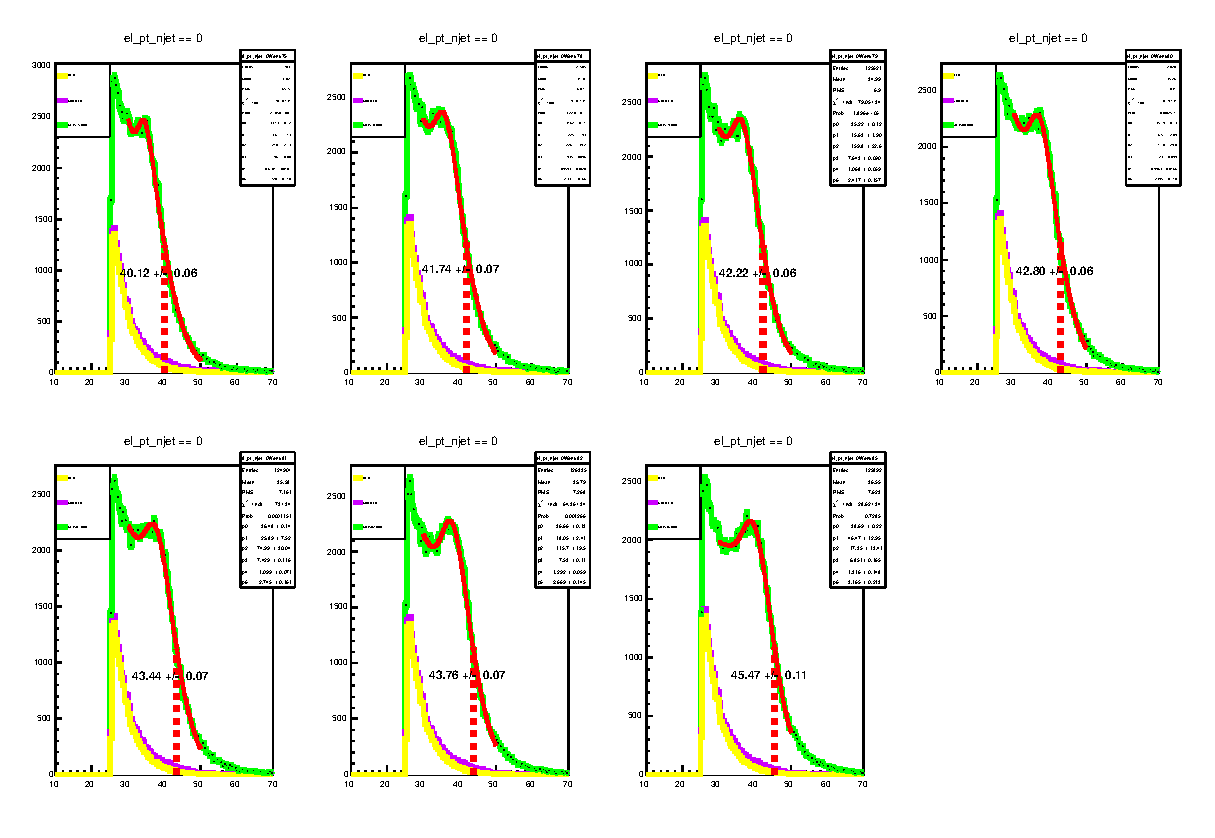
\includegraphics[width=\textwidth]{data/img/gauge_037.eps}
\caption{Gauge measurements for QCD scale factor 0.37 and fit range 30 - 50 GeV}
\end{figure}

\begin{figure}
\centering
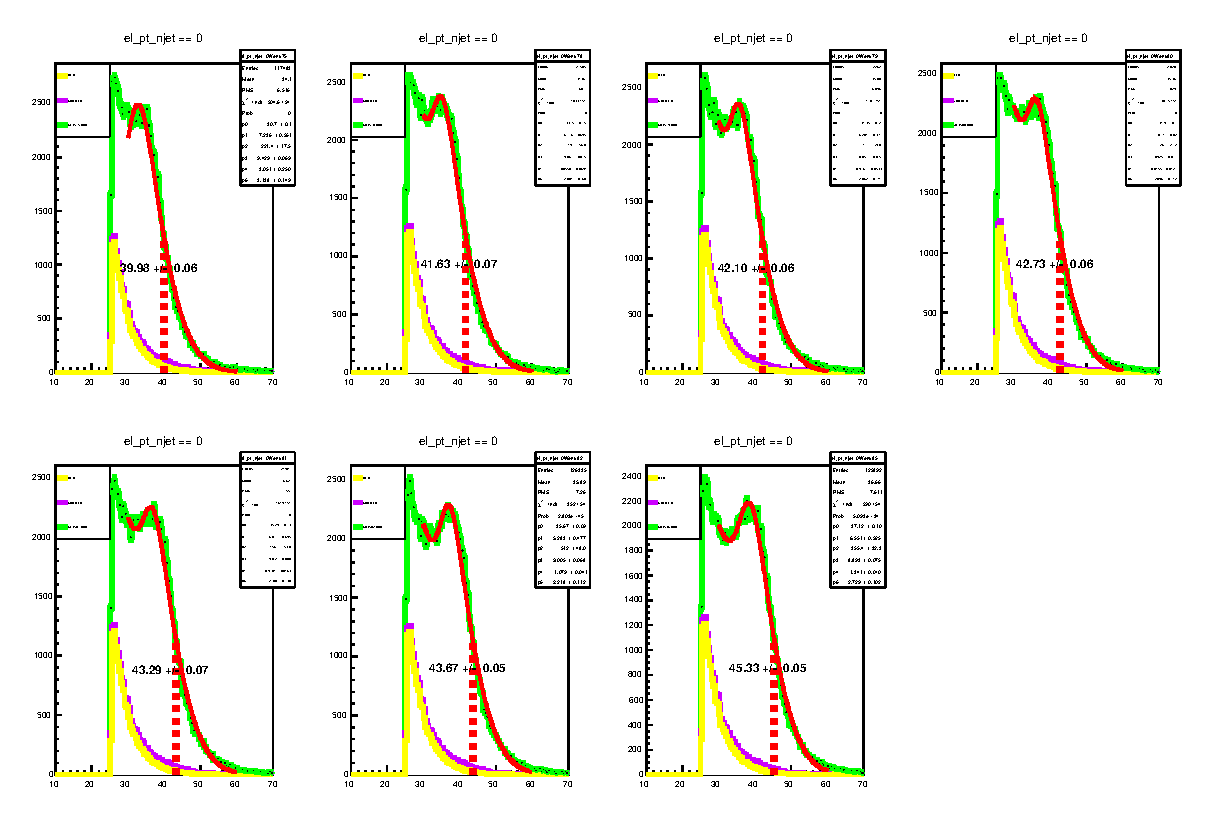
\includegraphics[width=\textwidth]{data/img/gauge_033_i_30_60.eps}
\caption{Gauge measurements for QCD scale factor 0.33 and fit range 30 - 60 GeV}
\end{figure}
\begin{figure}
\centering
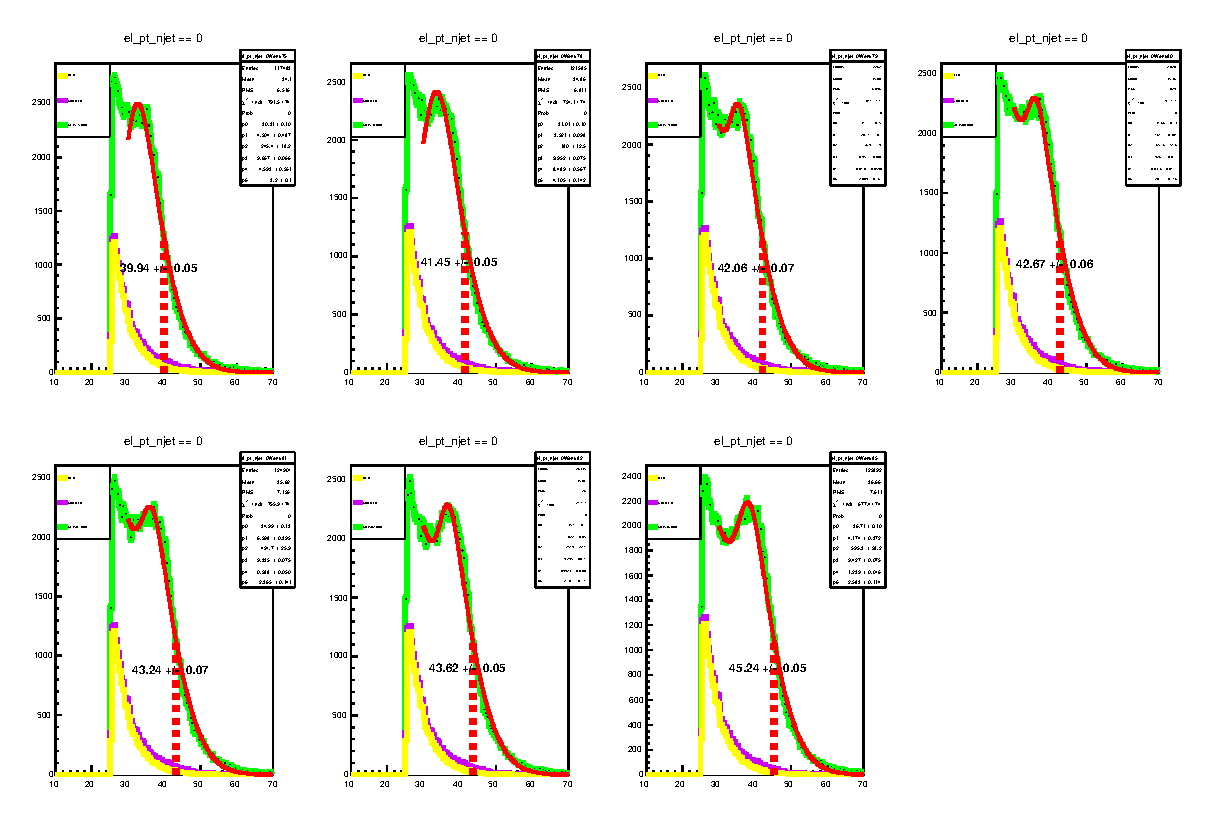
\includegraphics[width=\textwidth]{data/img/gauge_033_i_30_70.eps}
\caption{Gauge measurements for QCD scale factor 0.33 and fit range 30 - 70 GeV}
\end{figure}
\begin{figure}
\centering
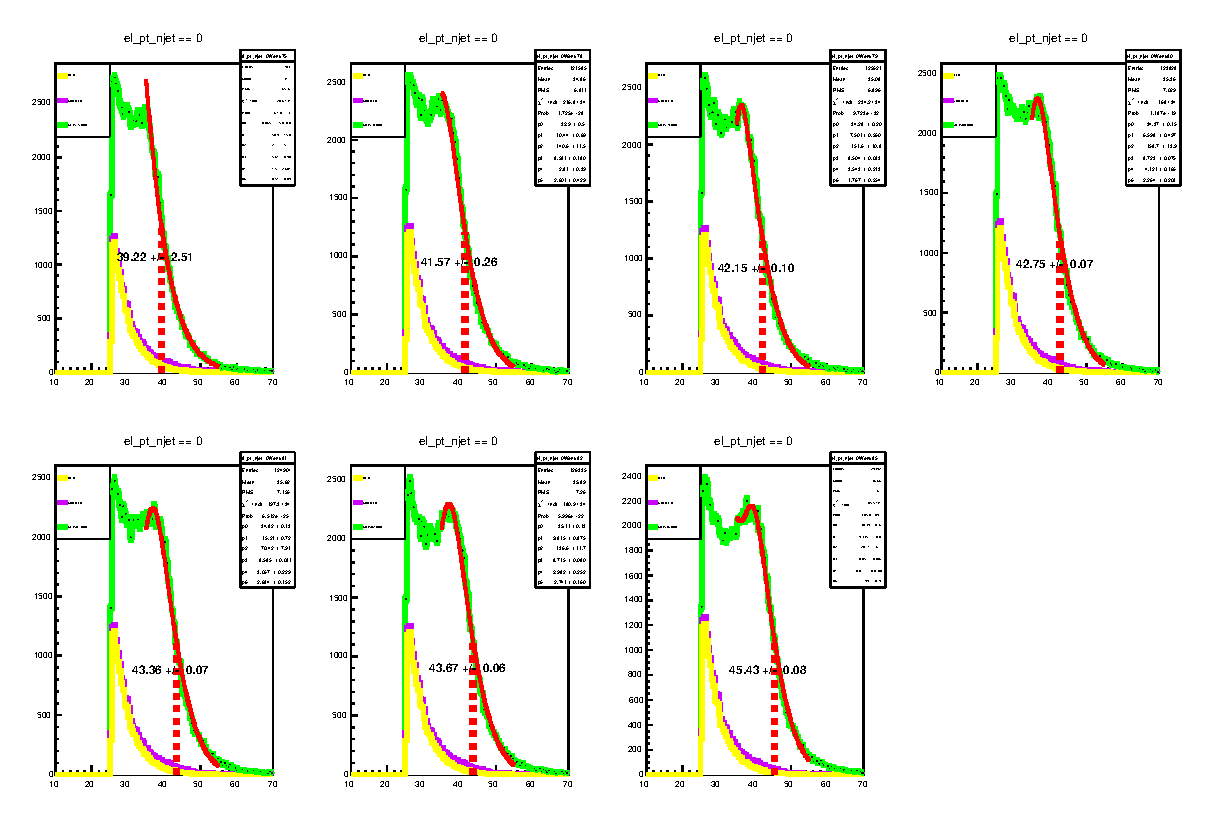
\includegraphics[width=\textwidth]{data/img/gauge_033_i_35_55.eps}
\caption{Gauge measurements for QCD scale factor 0.33 and fit range 35 - 55 GeV}
\end{figure}

\subsection{Wenu dataset fits}
\begin{figure}
\centering
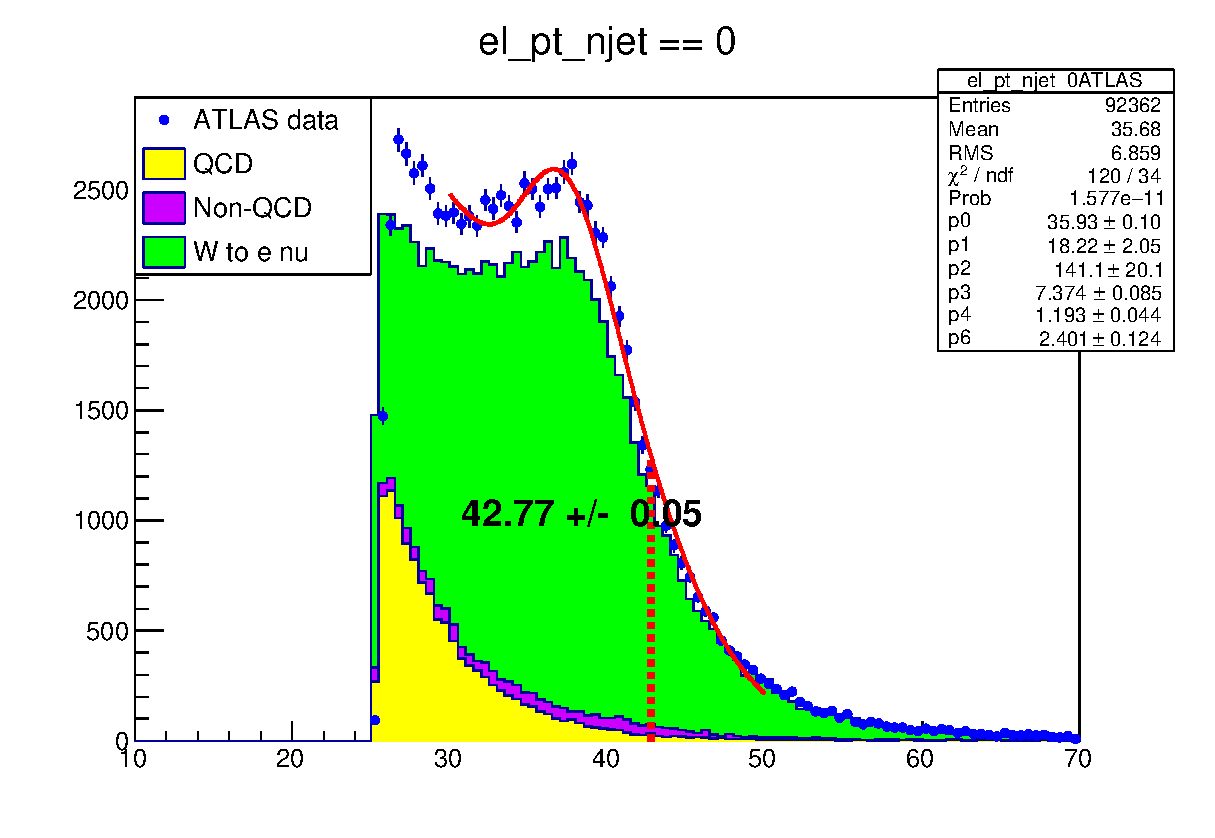
\includegraphics[width=\textwidth]{data/img/halfmax_Wenu_031.eps}
\caption{Fit to Wenu data for QCD scale factor 0.31 and fit range 30 - 50 GeV}
\end{figure}
\begin{figure}
\centering
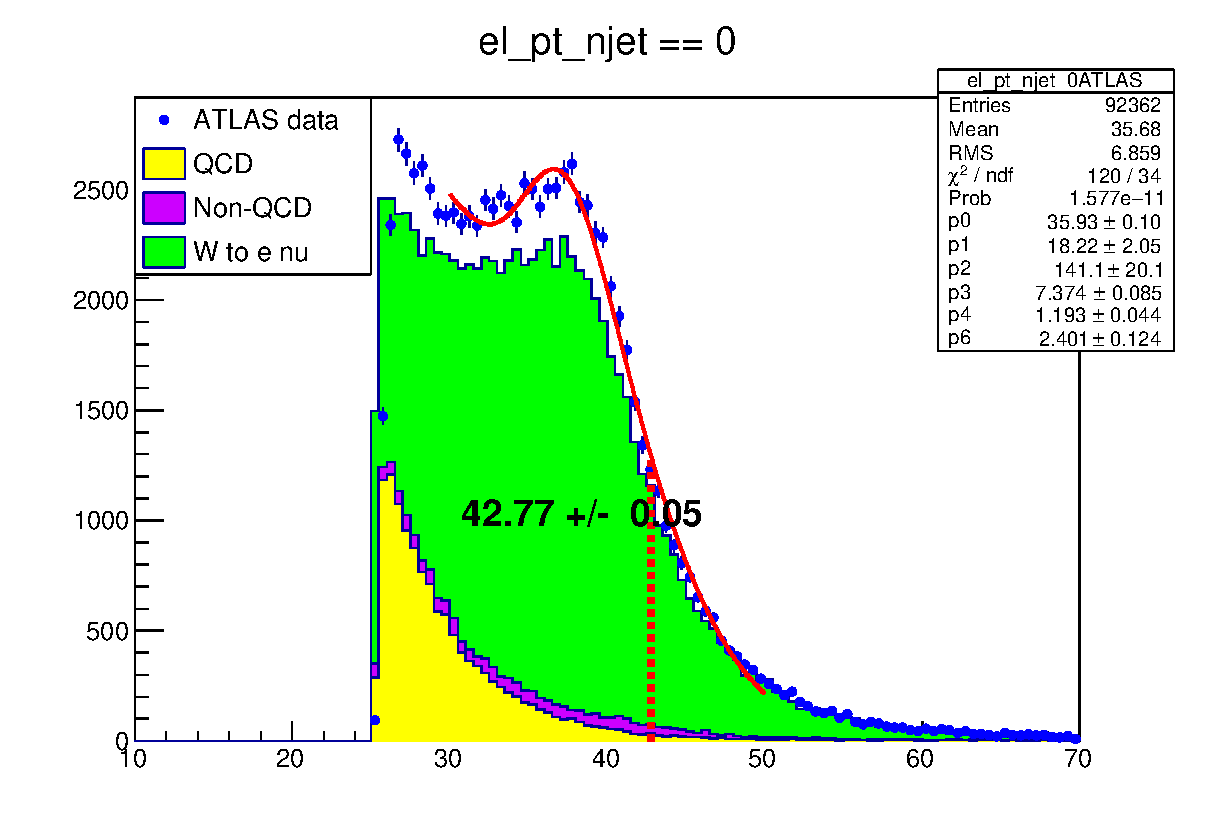
\includegraphics[width=\textwidth]{data/img/halfmax_Wenu_033.eps}
\caption{Fit to Wenu data for QCD scale factor 0.33 and fit range 30 - 50 GeV}
\end{figure}
\begin{figure}
\centering
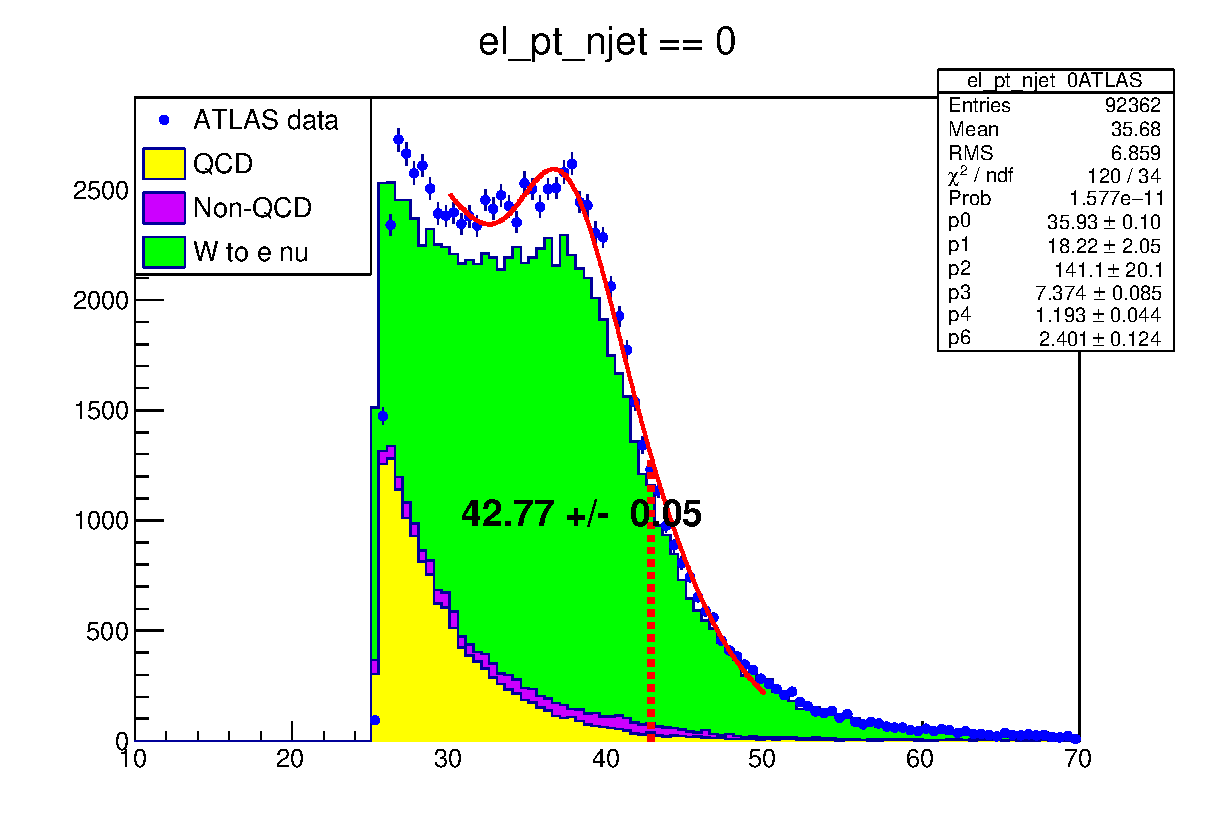
\includegraphics[width=\textwidth]{data/img/halfmax_Wenu_035.eps}
\caption{Fit to Wenu data for QCD scale factor 0.35 and fit range 30 - 50 GeV}
\end{figure}
\begin{figure}
\centering
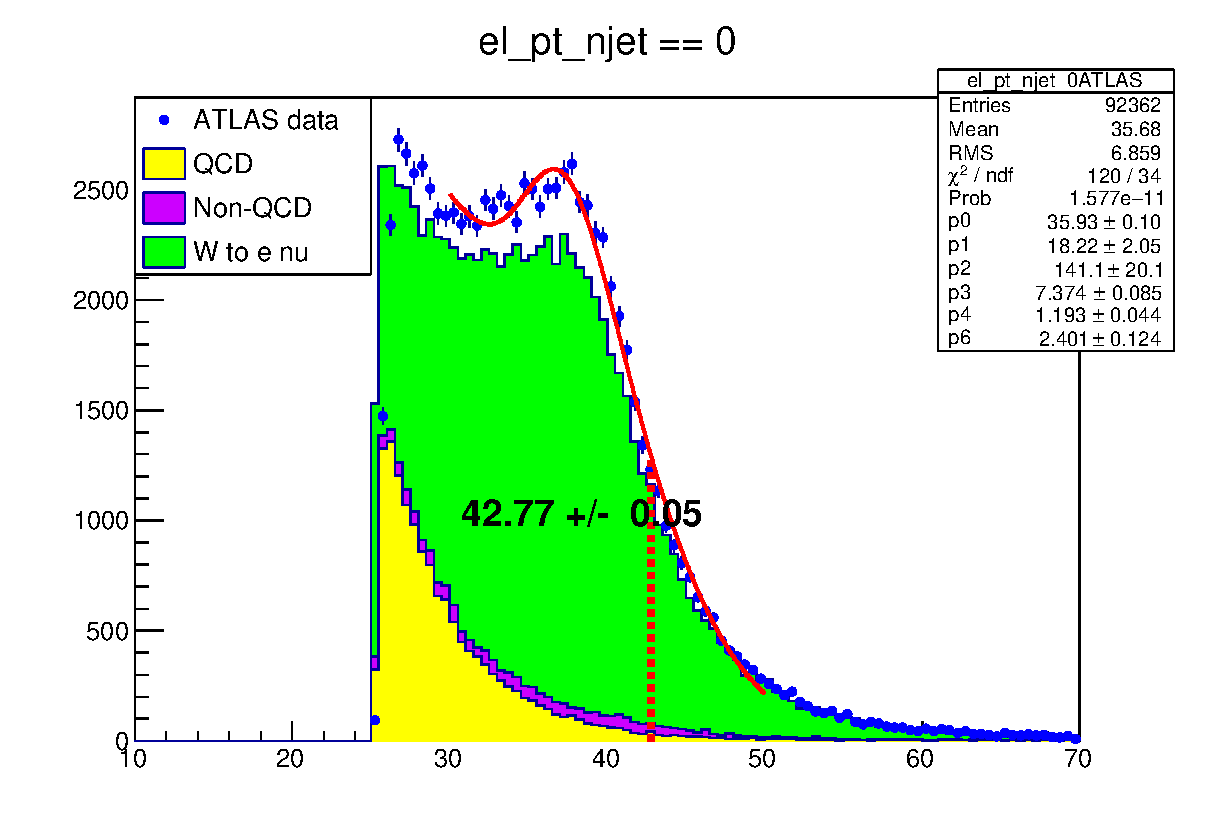
\includegraphics[width=\textwidth]{data/img/halfmax_Wenu_037.eps}
\caption{Fit to Wenu data for QCD scale factor 0.37 and fit range 30 - 50 GeV}
\end{figure}

\begin{figure}
\centering
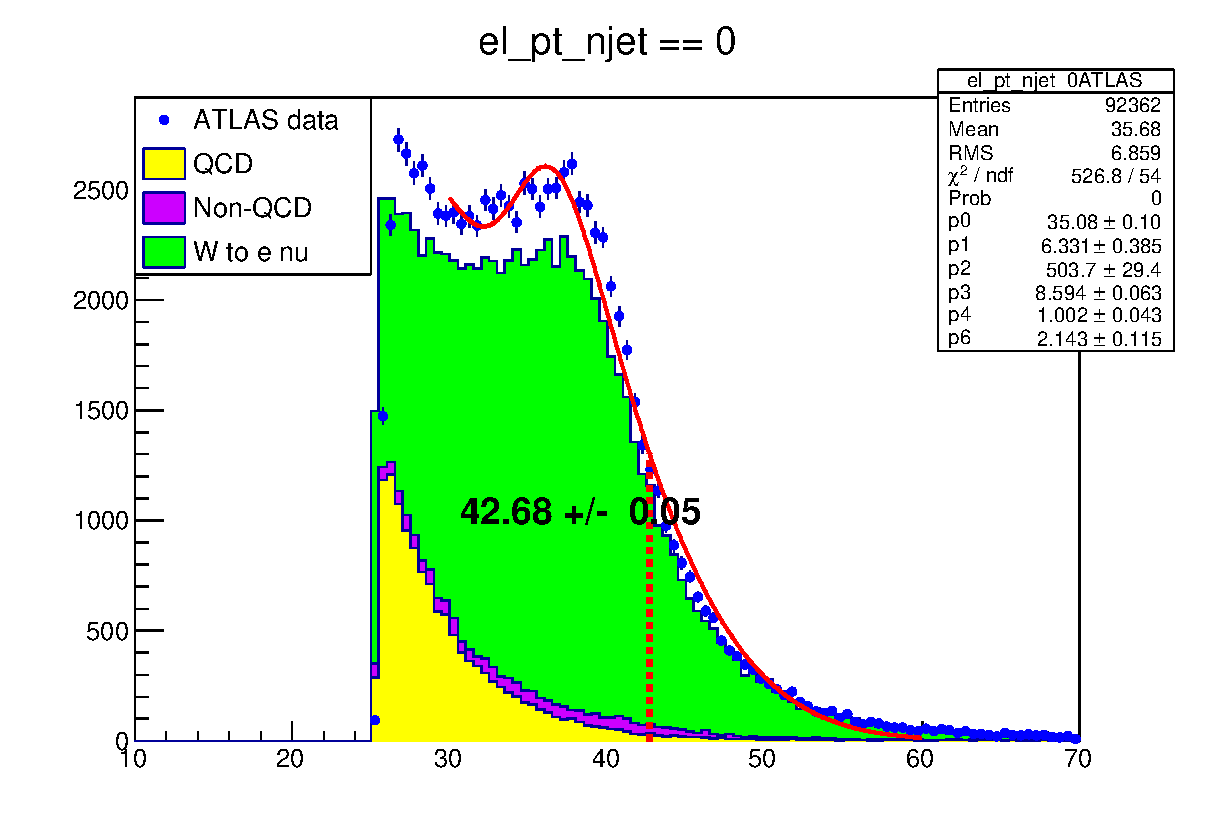
\includegraphics[width=\textwidth]{data/img/halfmax_Wenu_033_i_30_60.eps}
\caption{Fit to Wenu data for QCD scale factor 0.33 and fit range 30 - 60 GeV}
\end{figure}
\begin{figure}
\centering
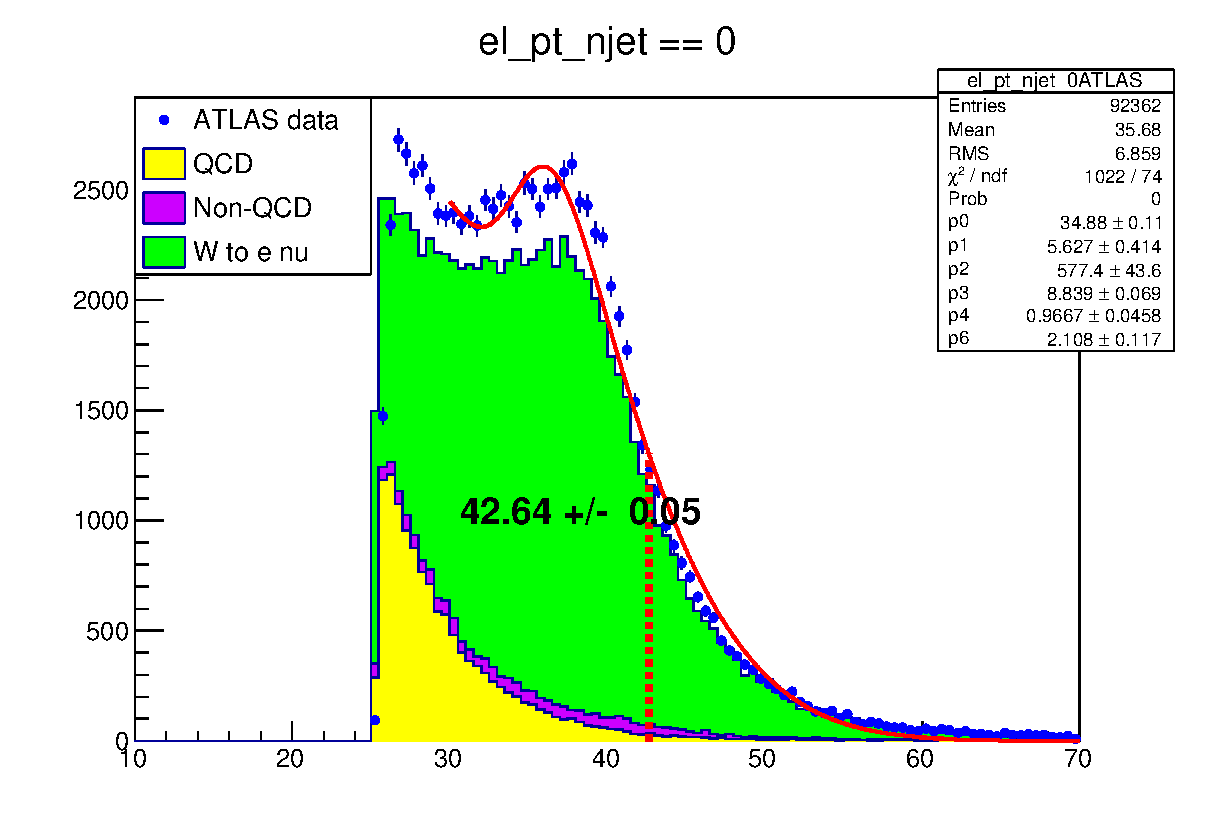
\includegraphics[width=\textwidth]{data/img/halfmax_Wenu_033_i_30_70.eps}
\caption{Fit to Wenu data for QCD scale factor 0.33 and fit range 30 - 70 GeV}
\end{figure}
\begin{figure}
\centering
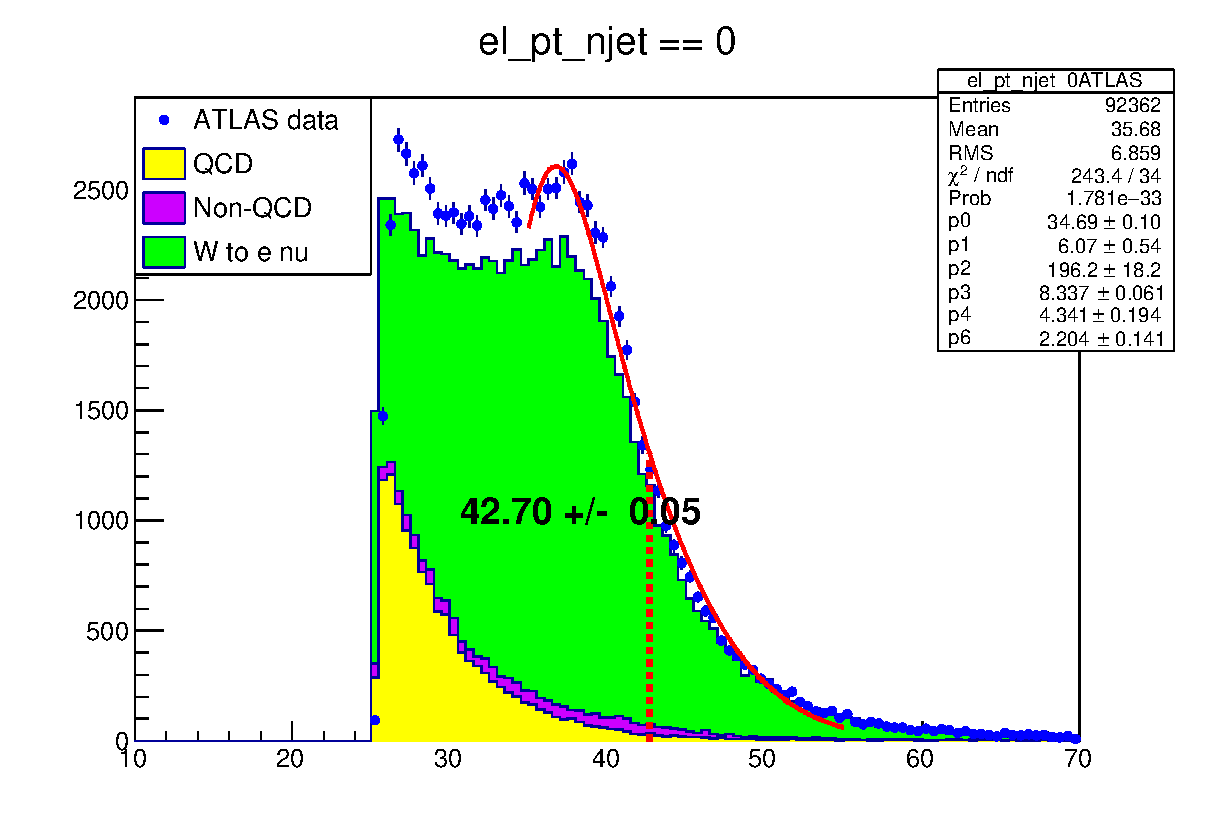
\includegraphics[width=\textwidth]{data/img/halfmax_Wenu_033_i_35_55.eps}
\caption{Fit to Wenu data for QCD scale factor 0.33 and fit range 35 - 55 GeV}
\end{figure}

\subsection{Zee dataset fit}
\begin{figure}
\centering
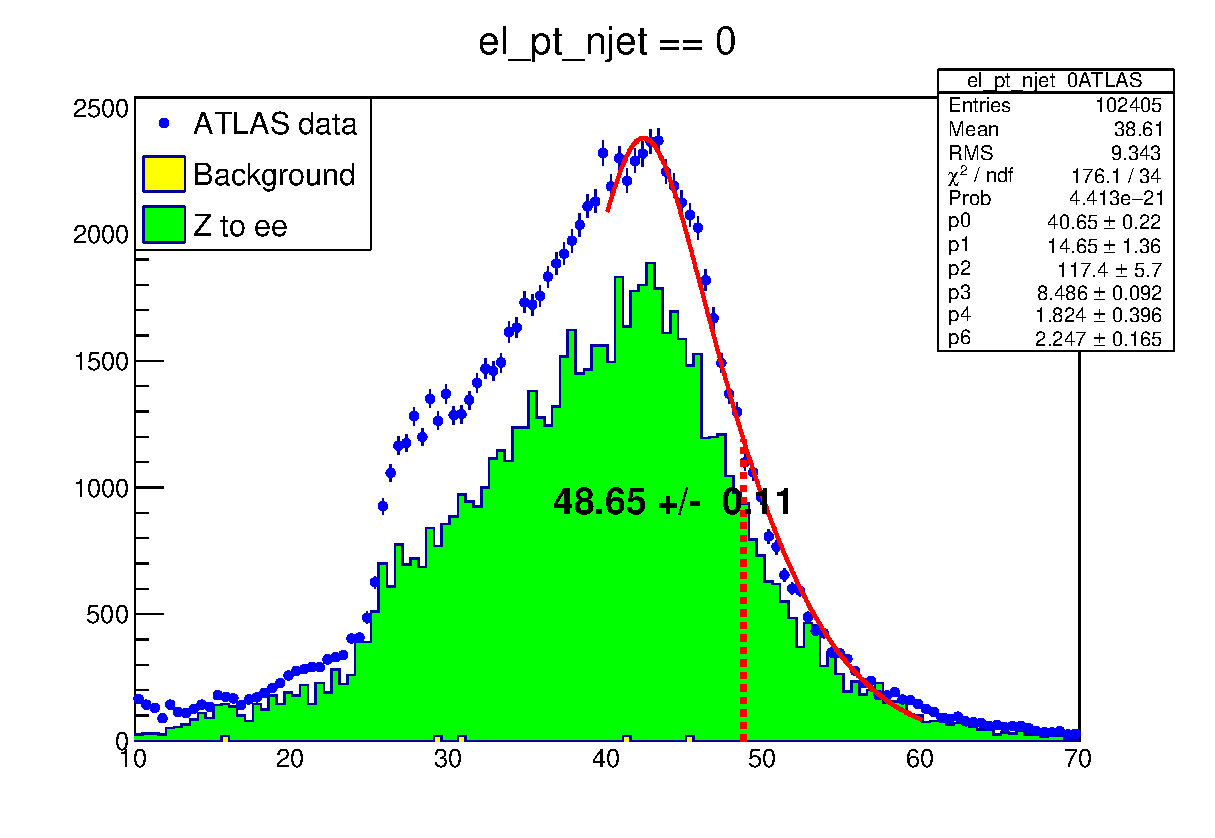
\includegraphics[width=\textwidth]{data/img/halfmax_Zee_033.eps}
\caption{Fit to Zee data for QCD scale factor 0.33 and fit range 30 - 50 GeV}
\end{figure}

\end{document}
